%================================================================
\section{Results and Discussion}\label{sec:Results}
%================================================================

The programs containing the implementation of the methods discussed in the previous section, as well as the results presented in this section, can be found at the GitHub repository
\begin{center}
    \url{https://github.com/nicolossus/FYS-STK4155-Project2}
\end{center}

The procedures for producing the following results are contained in Jupyter Notebooks found \href{https://github.com/nicolossus/FYS-STK4155-Project2/tree/master/notebooks}{here}.

%----------------------------------------------------------------
\subsection{Learning the Ising Hamiltonian with Linear Regression}\label{sec:results linreg}
%----------------------------------------------------------------
Accompanying notebook: \href{https://github.com/nicolossus/FYS-STK4155-Project2/blob/master/notebooks/linreg_ising.ipynb}{linreg\_ising.ipynb}.

\autoref{fig:j_ols} shows the coupling matrix obtained by performing OLS regression.

\begin{figure}[H]
\begin{center}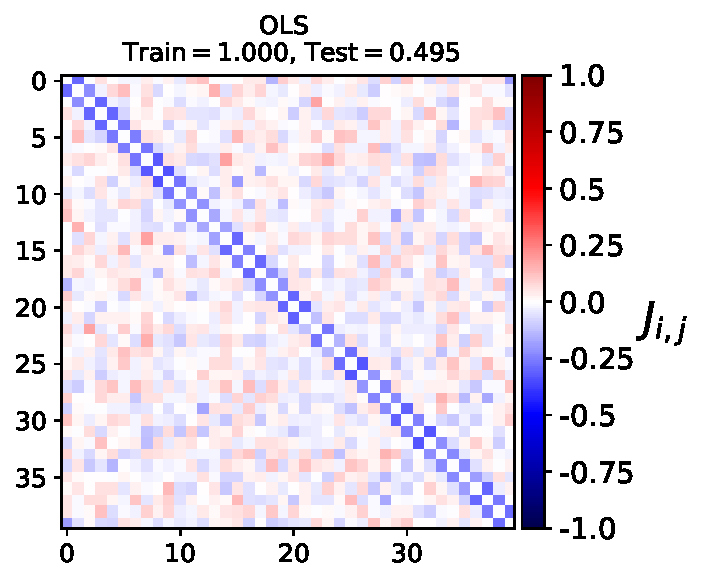
\includegraphics[scale=0.6]{latex/figures/ising_J_ols.pdf}
\end{center}
\caption{figure text}
\label{fig:j_ols}
\end{figure}

\autoref{fig:j_lmbda} shows the coupling matrices obtained by performing Ridge and Lasso regression with different regularization parameter, $\lambda$, values.

\begin{figure}[H]
\captionsetup[subfigure]{labelformat=empty}
\centering
\subfloat[]{{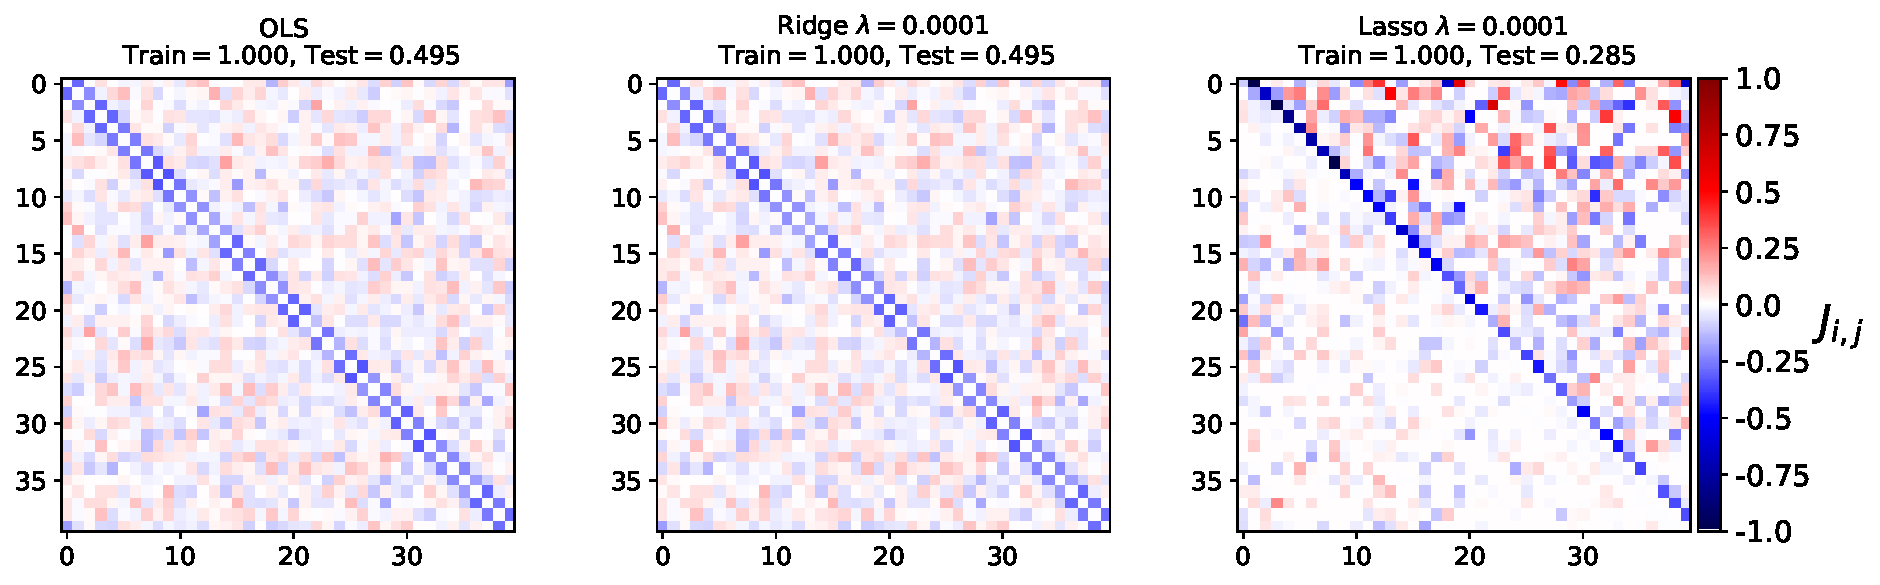
\includegraphics[scale=0.35]{latex/figures/ising_J_lmbda_0_0001.pdf}}}
\qquad
\subfloat[]{{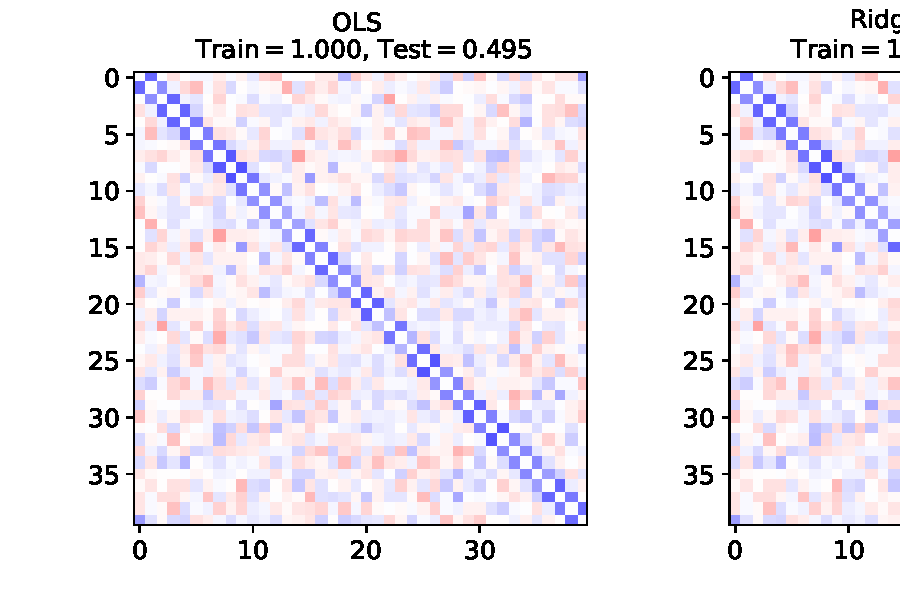
\includegraphics[scale=0.35]{latex/figures/ising_J_lmbda_0_001.pdf}}}
\qquad
\subfloat[]{{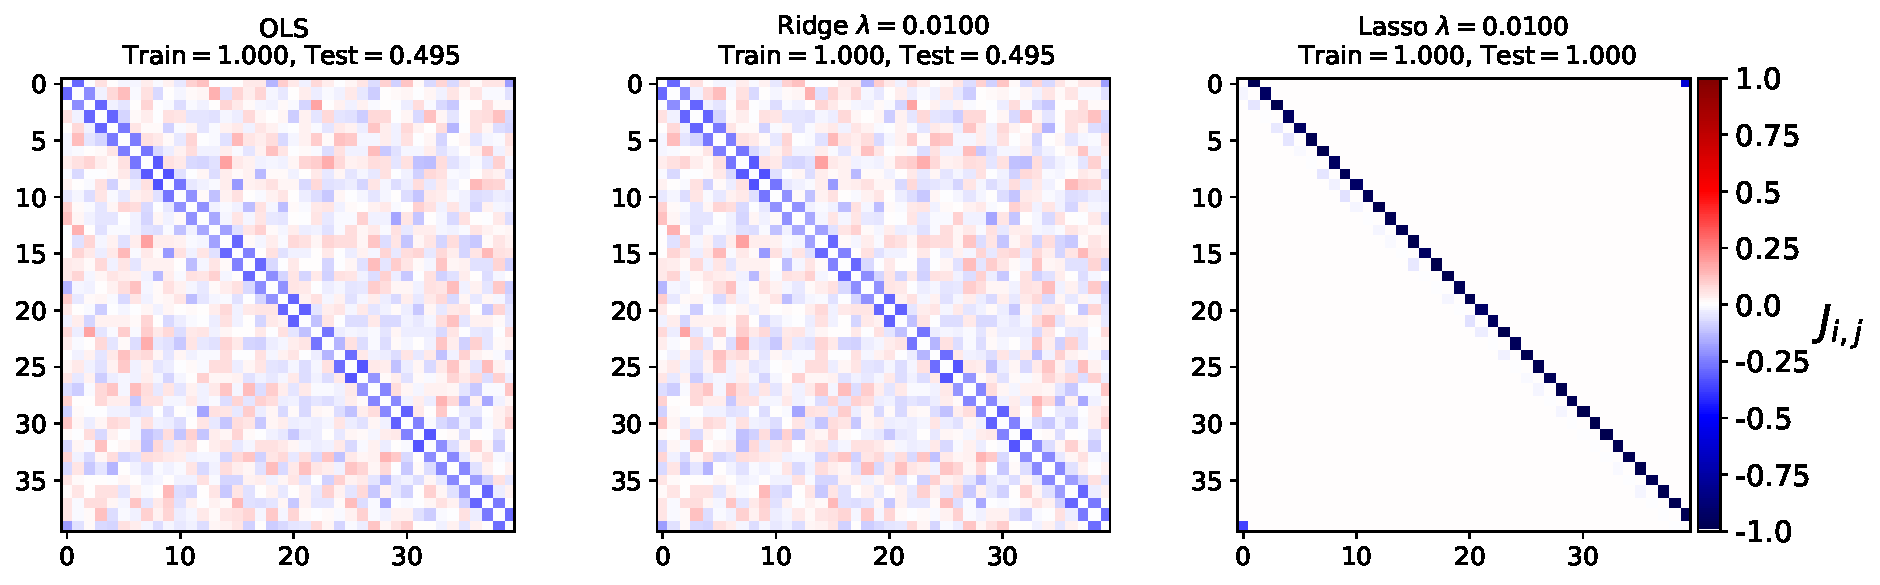
\includegraphics[scale=0.35]{latex/figures/ising_J_lmbda_0_01.pdf}}}
\qquad
\subfloat[]{{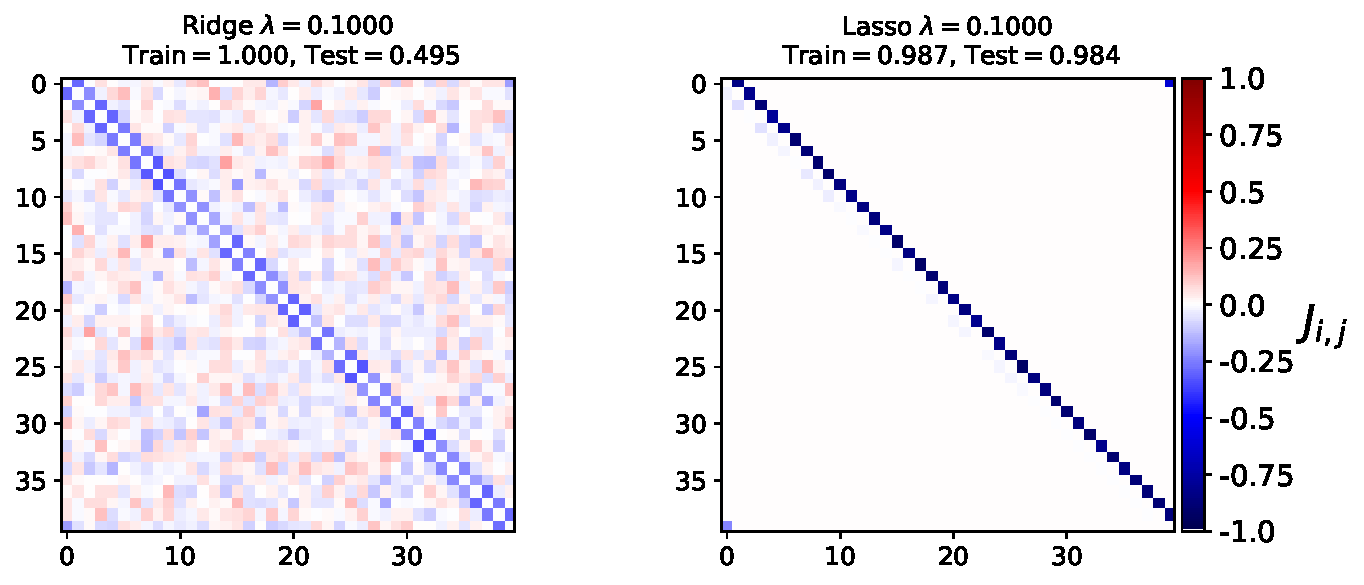
\includegraphics[scale=0.35]{latex/figures/ising_J_lmbda_0_1.pdf}}}
\qquad
\subfloat[]{{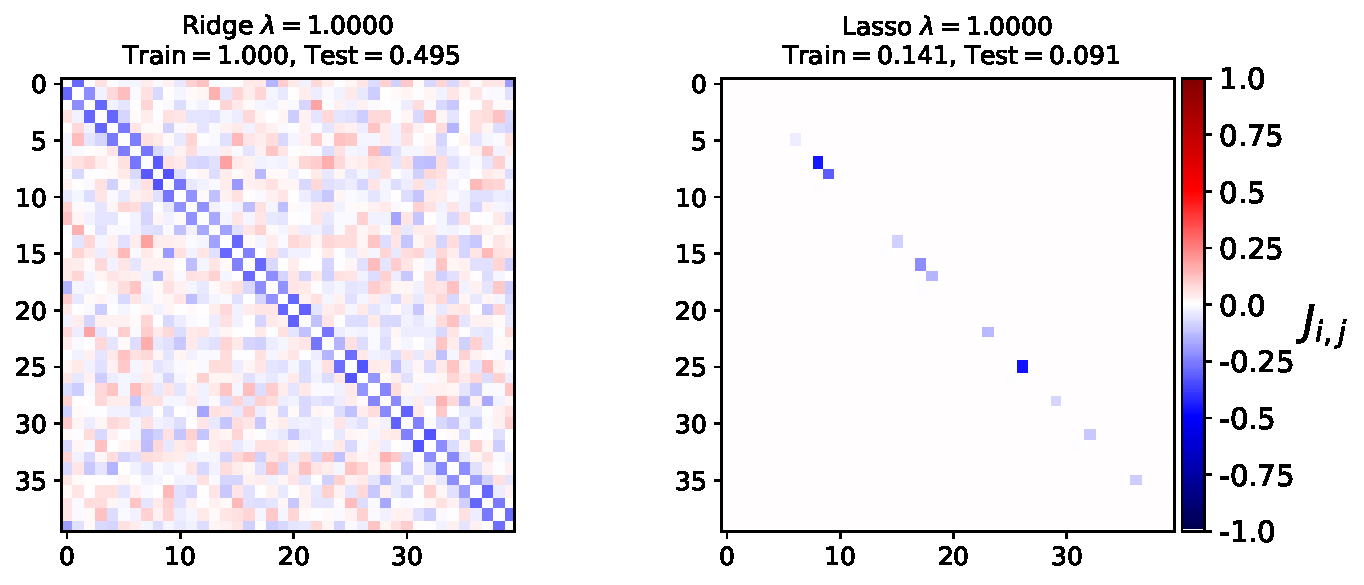
\includegraphics[scale=0.35]{latex/figures/ising_J_lmbda_1_0.pdf}}}
\qquad
\subfloat[]{{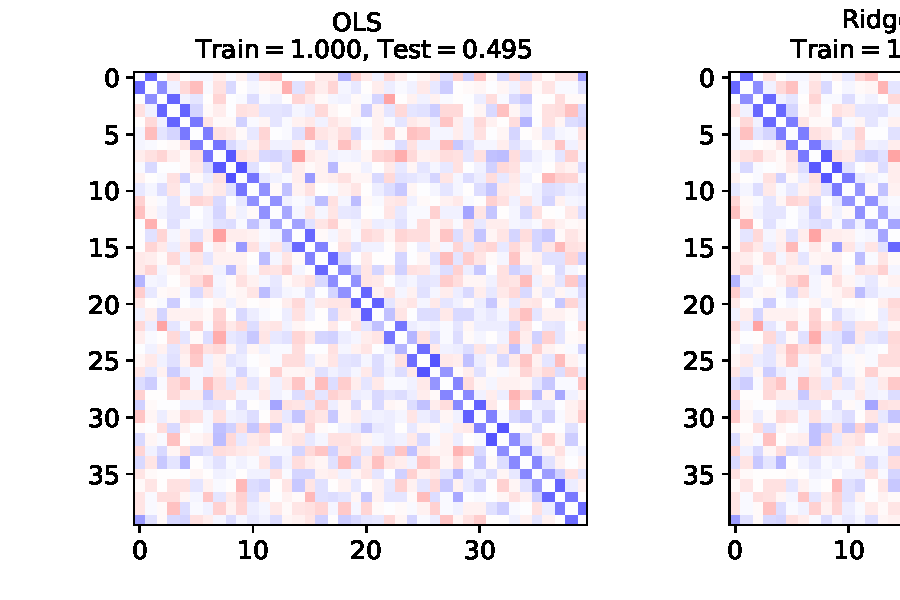
\includegraphics[scale=0.35]{latex/figures/ising_J_lmbda_10_0.pdf}}}
\qquad
\subfloat[]{{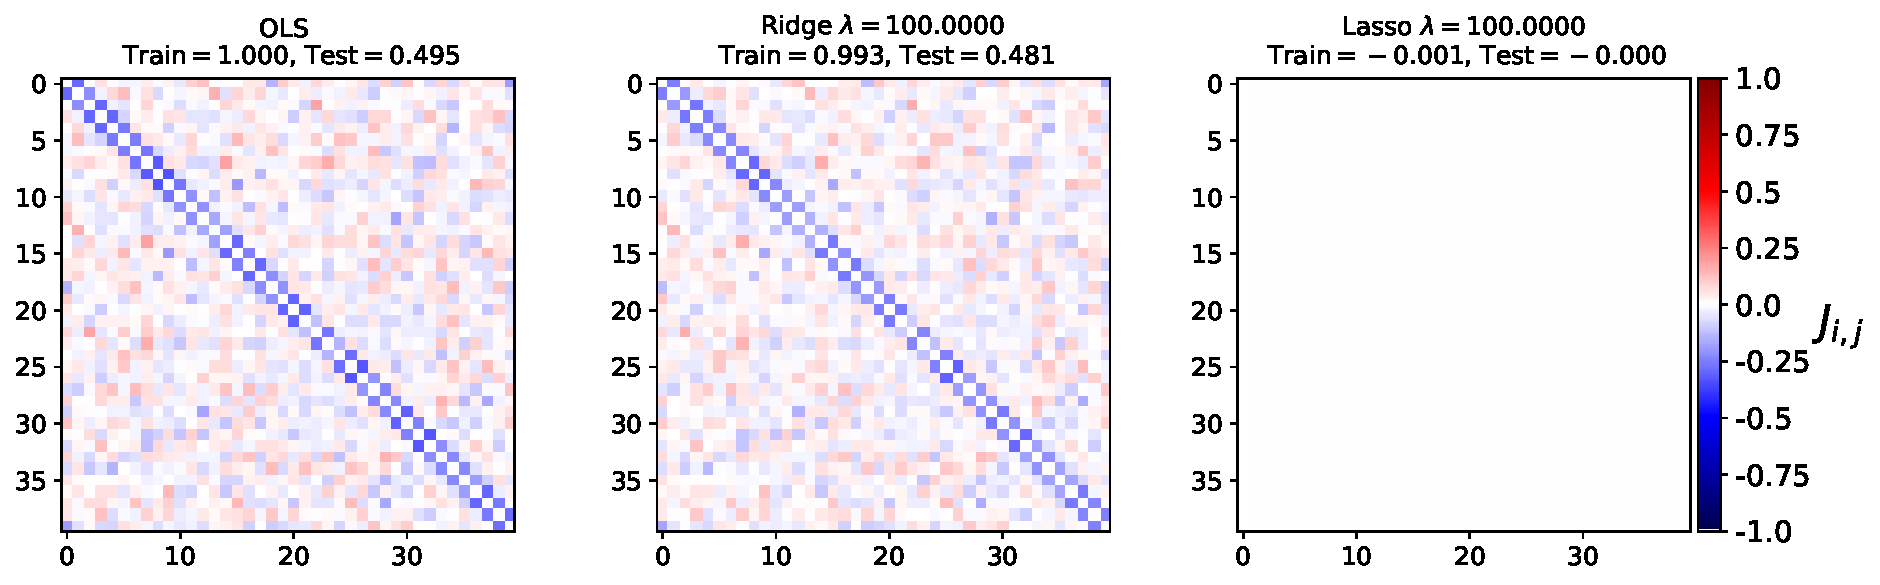
\includegraphics[scale=0.35]{latex/figures/ising_J_lmbda_100_0.pdf}}}
\qquad
\subfloat[]{{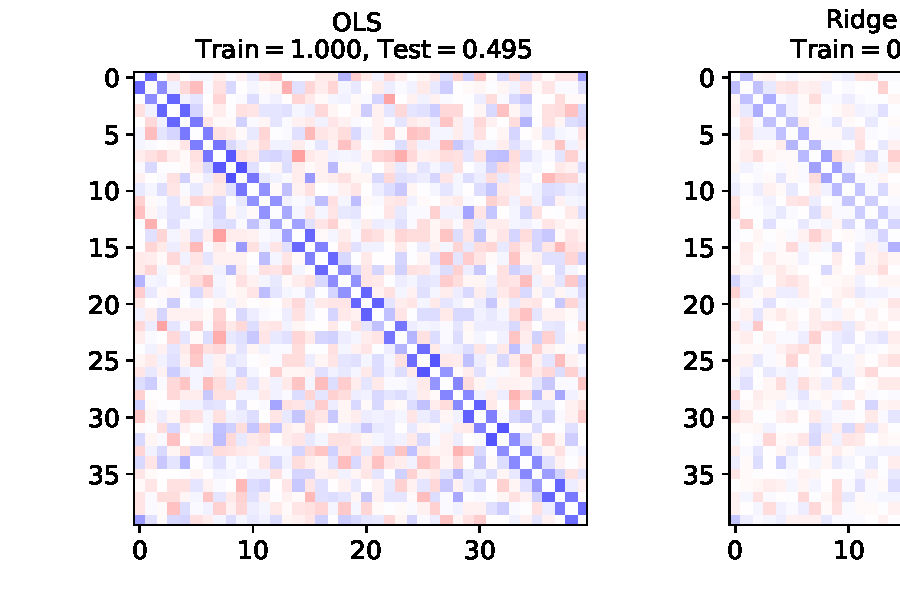
\includegraphics[scale=0.35]{latex/figures/ising_J_lmbda_1000_0.pdf}}}
\qquad
\subfloat[]{{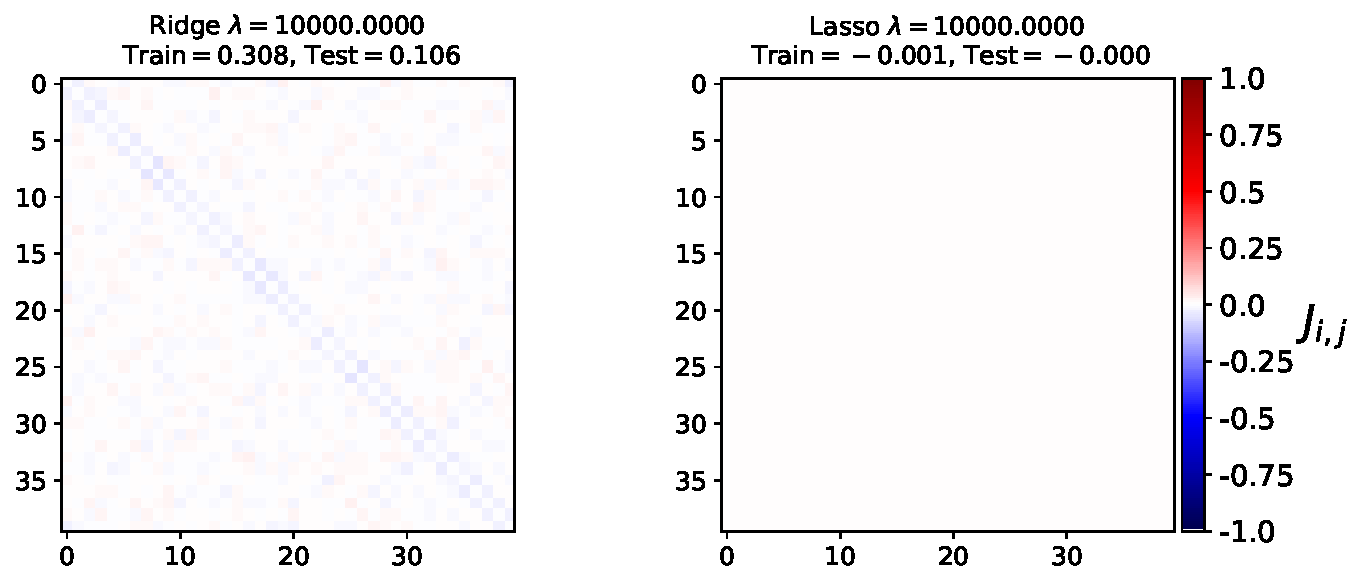
\includegraphics[scale=0.35]{latex/figures/ising_J_lmbda_10000_0.pdf}}}
\qquad
\subfloat[]{{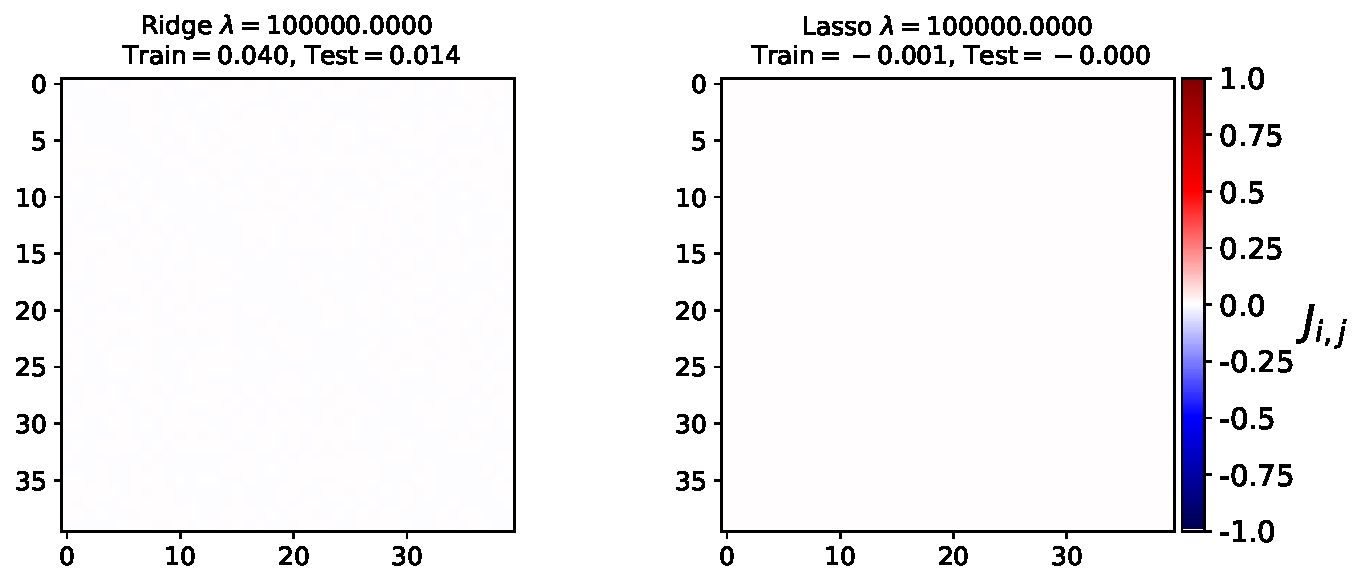
\includegraphics[scale=0.35]{latex/figures/ising_J_lmbda_100000_0.pdf}}}
\caption{figure text}
\label{fig:j_lmbda}
\end{figure}

When doing the regression we included both $s_j s_i$ and $s_i s_j$ for all $i,j$ in the features. Since these quantities are equal, we do not get a unique solution for OLS, so we resort to singular value decomposition (SVD). SVD gives the coefficients with the least $L2$-norm. Hence we tend to get solutions $J_{i,j}=J_{j,i}=-0.5$. Ridge is similar in this regard, since it uses an $L2$ penalty. Lasso uses the $L1$-norm which doesn't differentiate between e.g. $J_{i,j}=-1$ and $J_{j,i} = 0$ on one hand and $J_{i,j}=J_{j,i}=-0.5$ on the other. Lasso tends to give coefficients which are equal to zero, which is consistent with what we have observed here.


\autoref{fig:performance_lmbda_1d} shows the $R^2$ score and MSE as a function of the regularization parameter $\lambda$.

\begin{figure}[H]
\centering
\subfloat[]{{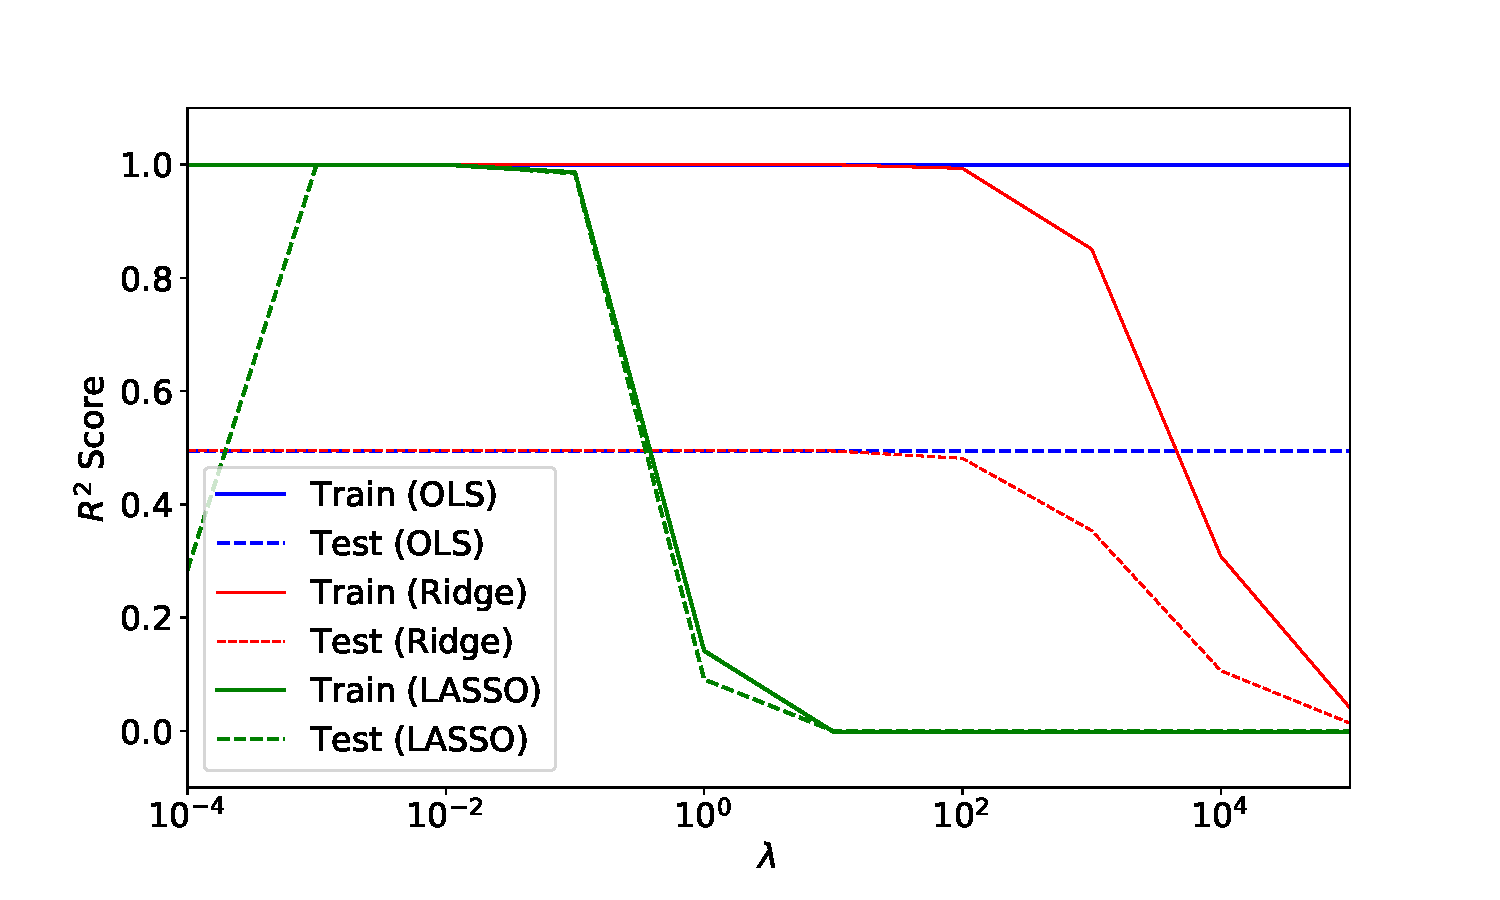
\includegraphics[scale=0.5]{latex/figures/ising1D_r2_vs_lmbda.pdf}}}
\qquad
\subfloat[]{{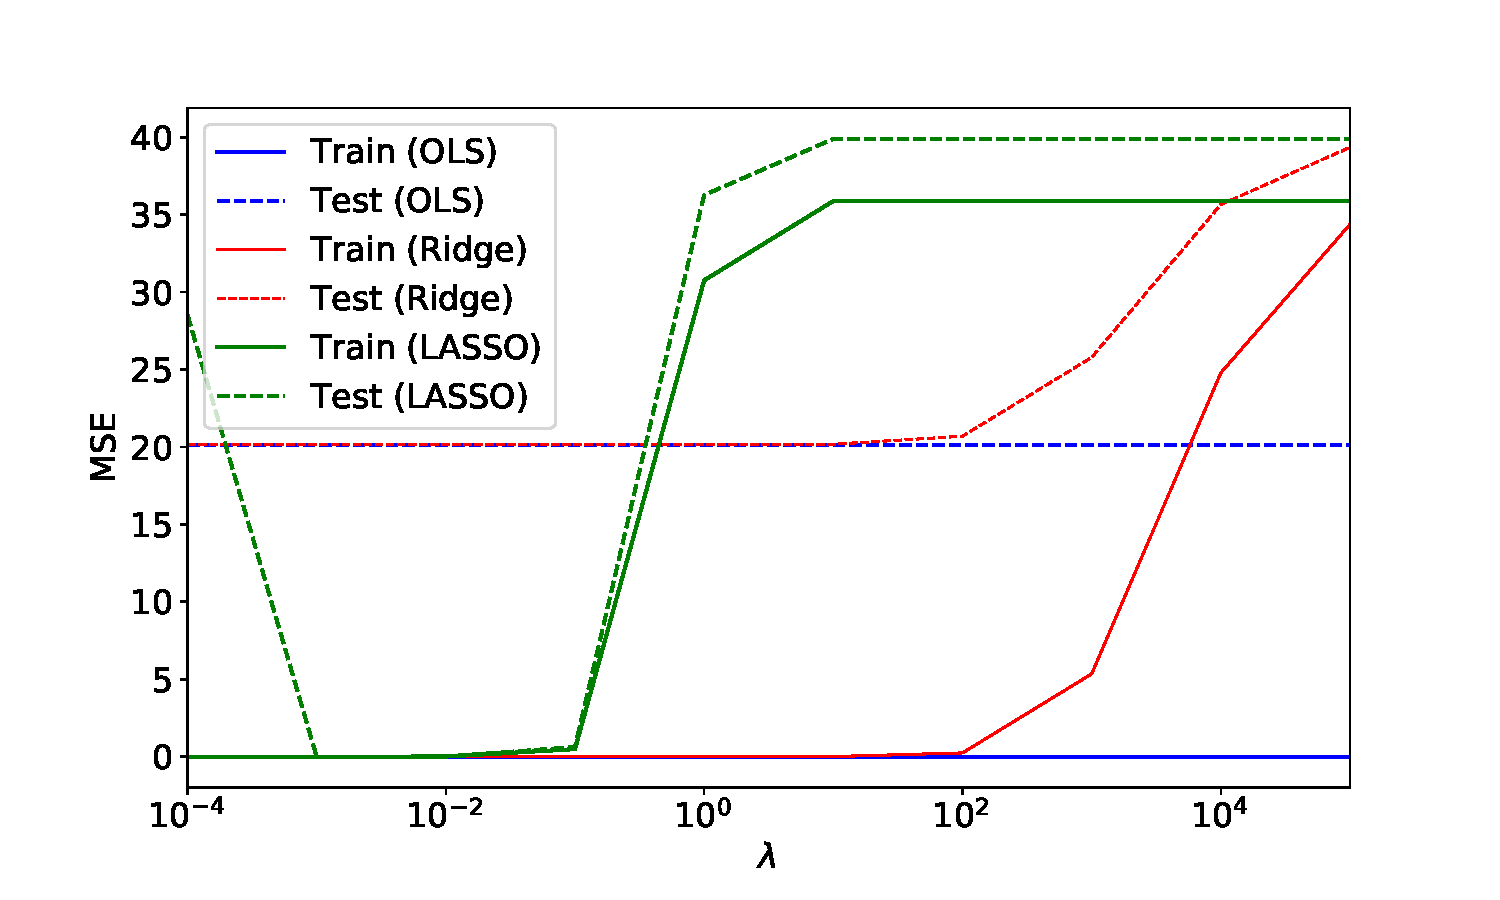
\includegraphics[scale=0.5]{latex/figures/ising1D_mse_vs_lmbda.pdf}}}
\caption{figure text}
\label{fig:performance_lmbda_1d}
\end{figure}

DISCUSS R2 MSE

BIAS-VARIANCE

%----------------------------------------------------------------
\subsection{Identifying 2D Ising Model Phases with Logistic Regression}\label{sec:results logreg}
%----------------------------------------------------------------
Accompanying notebook: \href{https://github.com/nicolossus/FYS-STK4155-Project2/blob/master/notebooks/logreg_ising.ipynb}{logreg\_ising.ipynb}. 

blablabla
5200 train samples
30000 critical samples
124800 test samples
table of (constant) parameters, n-iter

\begin{table}[H]
\caption{Table text}
\centering
\rowcolors{2}{gray!25}{white}
\begin{tabular}{ccc}
\hline
\hline 
$\alpha$ & $\beta$ & $\gamma$
\\
\hline 
\hline 
0.1 & 0.2 & 0.3
\\
0.4 & 0.5 & 0.6
\\
0.7 & 0.8 & 0.9
\\
\hline
\end{tabular}
\label{tab:tab1}
\end{table}


Optimal parameters, figures of acc 

\autoref{fig:gd_acc_lambda}

\begin{figure}[H]
\centering
\subfloat[]{{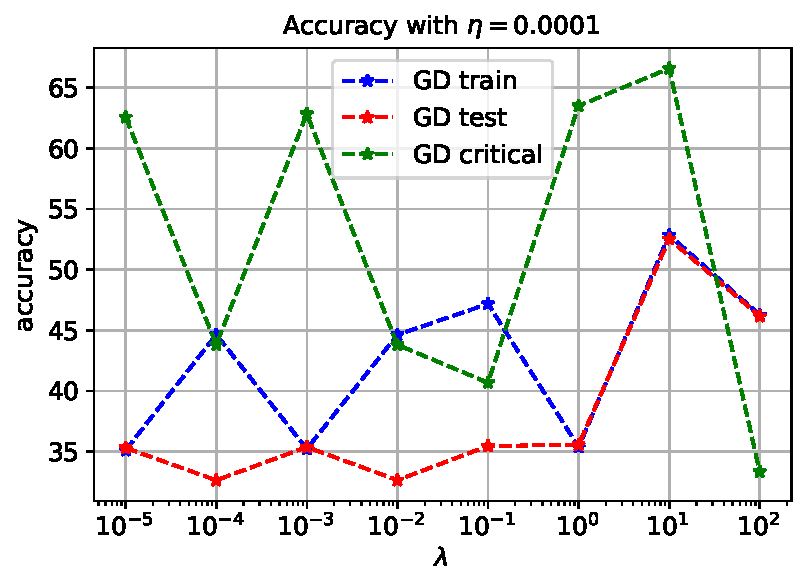
\includegraphics[scale=0.55]{latex/figures/log_acc_eta_0_0001.pdf}}}
\qquad
\subfloat[]{{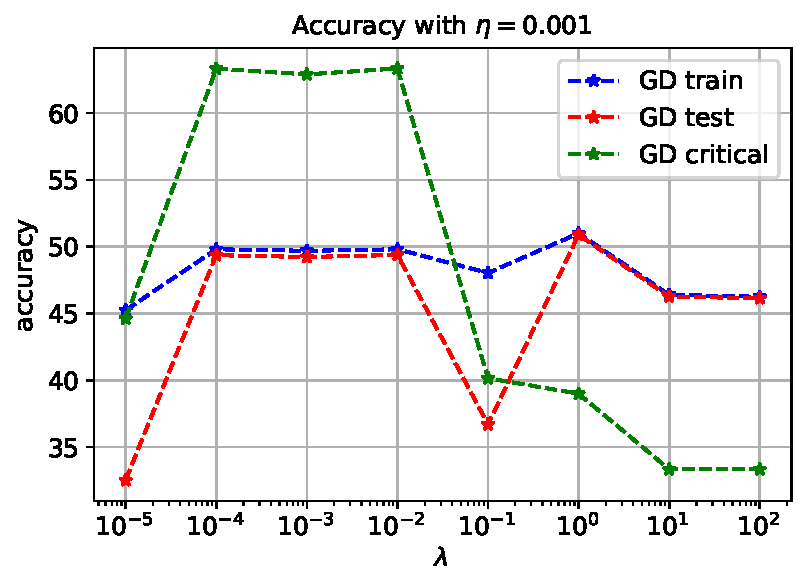
\includegraphics[scale=0.55]{latex/figures/log_acc_eta_0_001.pdf}}}
\qquad
\subfloat[]{{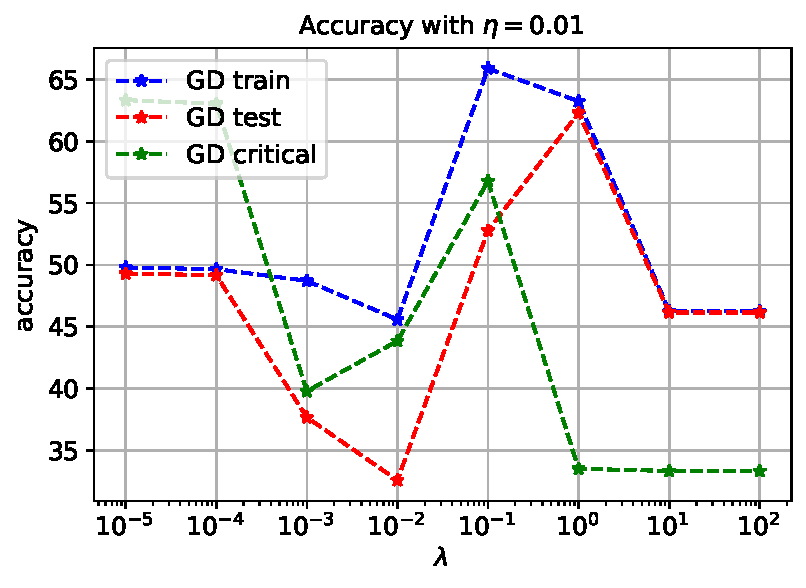
\includegraphics[scale=0.55]{latex/figures/log_acc_eta_0_01.pdf}}}
\qquad
\subfloat[]{{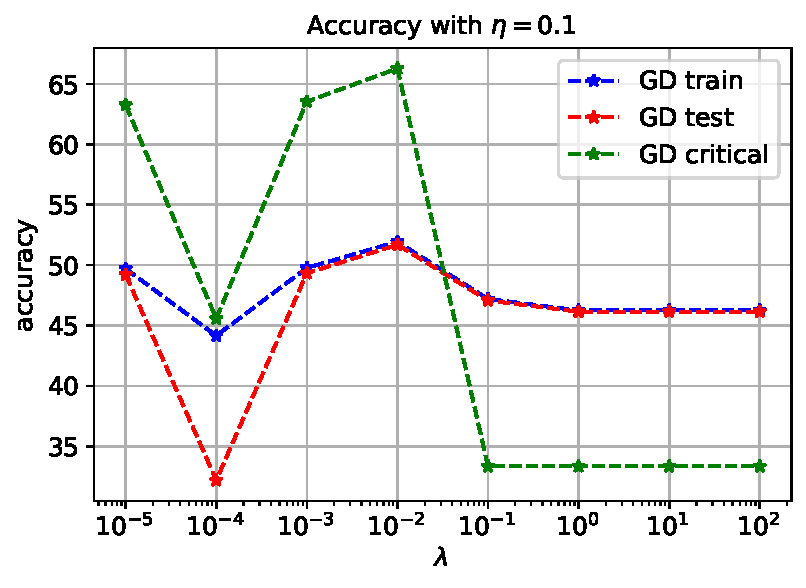
\includegraphics[scale=0.55]{latex/figures/log_acc_eta_0_1.pdf}}}
\caption{The accuracy score of the training, test and critical datasets as a function of the regularization parameter $\lambda$ for different learning rates $\eta$. Gradient descent was used as optimization method.}
\label{fig:gd_acc_lambda}
\end{figure}

COMMENT FIGURE

To easier see the actual values, \autoref{tab:opt params train}, \autoref{tab:opt params test} and \autoref{tab:opt params crit} tabulates the maximum accuracy for the training, test and critical dataset, respectively. All tables also lists the value of the parameters as well as the accuracy score of the other two datasets. The full table from which these were retrieved can be found in as \autoref{tab:full table} in \autoref{sec:Appendix B}.

\begin{table}[H]
\parbox{.45\linewidth}{
\caption{Maximum accuracy score for training dataset with the corresponding parameters listed and the accuracy score of the other two datasets listed as well.}
\centering
\rowcolors{2}{gray!25}{white}
\begin{tabular}{c}
\hline \hline
      20 \\
\hline \hline
 0.01000 \\
 0.10000 \\
65.88462 \\
52.76923 \\
56.78000 \\
\hline \hline
\end{tabular}

\label{tab:opt params train}
}
\hfill
\parbox{.45\linewidth}{
\caption{Maximum accuracy score for test dataset with the corresponding parameters listed and the accuracy score of the other two datasets listed as well.}
\centering
\rowcolors{2}{gray!25}{white}
\begin{tabular}{c}
\hline \hline
{} &       21 \\
\hline \hline
$\eta$            &  0.01000 \\
$\lambda$         &  1.00000 \\
Training accuracy & 63.23077 \\
Test accuracy     & 62.29567 \\
Critical accuracy & 33.51333 \\
\hline \hline
\end{tabular}

\label{tab:opt params test}
}
\end{table}


\begin{table}[H]
\caption{Maximum accuracy score for critical dataset with the corresponding parameters listed and the accuracy score of the other two datasets listed as well.}
\centering
\rowcolors{2}{gray!25}{white}
\begin{tabular}{cc}
\hline \hline
Table index &        6 \\
\hline \hline
$\eta$            &  0.00010 \\
$\lambda$         & 10.00000 \\
Training accuracy & 52.84615 \\
Test accuracy     & 52.51843 \\
Critical accuracy & 66.57667 \\
\hline \hline
\end{tabular}

\label{tab:opt params crit}
\end{table}

There are no clear optimal parameters, and the accuracy with a particular set of parameters also changes for different runs. None of the best accuracies are great either. However, we stick with the best result for the maximum training accuracy in the table above on a larger training set (20\%). The results are shown in table

26000 train samples
30000 critical samples
104000 test samples
eta: 0.01
lambda: 0.1
Training accuracy 53.74230769230769
Test accuracy 53.61057692307693
Critical accuracy 66.66666666666666

A roc curve tells us more. Roc curve in figure ..

\autoref{fig:roc_gd}

\begin{figure}[H]
\begin{center}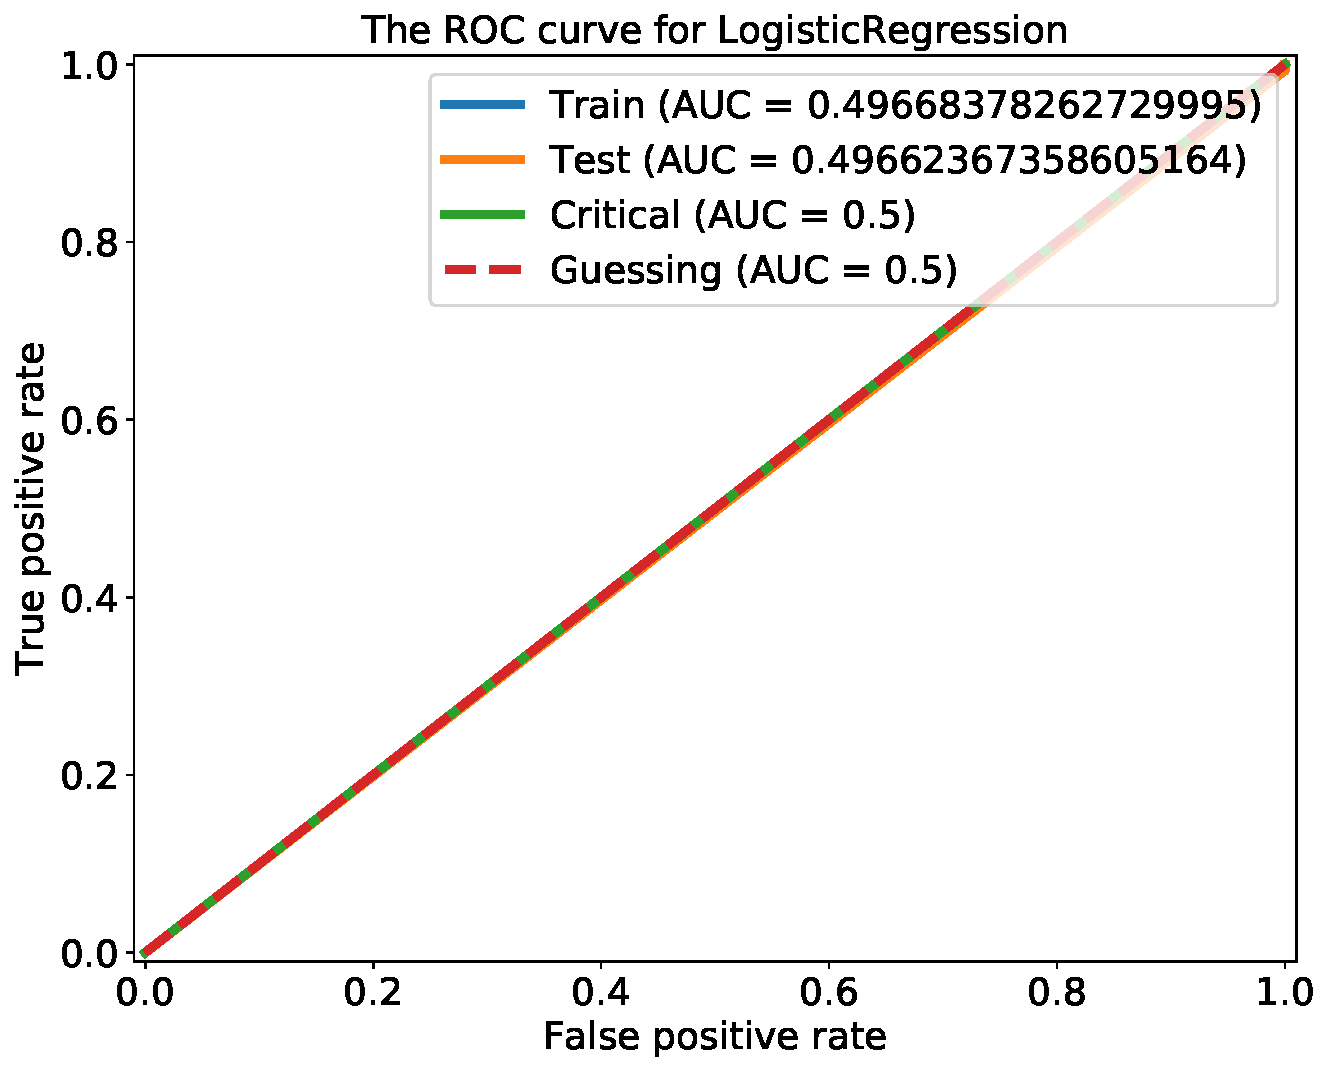
\includegraphics[scale=0.5]{latex/figures/logistic_roc_curve_gd.pdf}
\end{center}
\caption{figure text}
\label{fig:roc_gd}
\end{figure}

As seen in the figure, our logistic regression model with gradient descent does no better than just guessing the phase.

A second optimization method has also been implemented, NR.
This method is notoriously slow iterative scheme, so we will only apply it on a small training set and with few iterations. Only 4\% training data and 5 iterations 

table of parameters

best regularization parameter

\autoref{fig:acc_nr}

\begin{figure}[H]
\begin{center}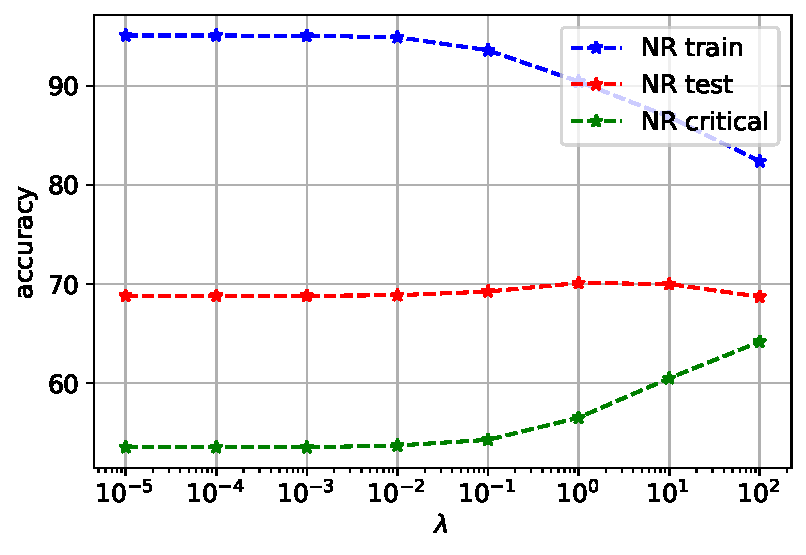
\includegraphics[scale=0.7]{latex/figures/log_acc_nr.pdf}
\end{center}
\caption{figure text}
\label{fig:acc_nr}
\end{figure}

$\lambda = 10^2$ clearly gives the highest accuracy when all states are taken into account. As the training and test accuracy is declining for this $\lambda$, this seems like an optimal value. We therefore plot the ROC curve with this regularization.

\autoref{fig:roc_nr}

\begin{figure}[H]
\begin{center}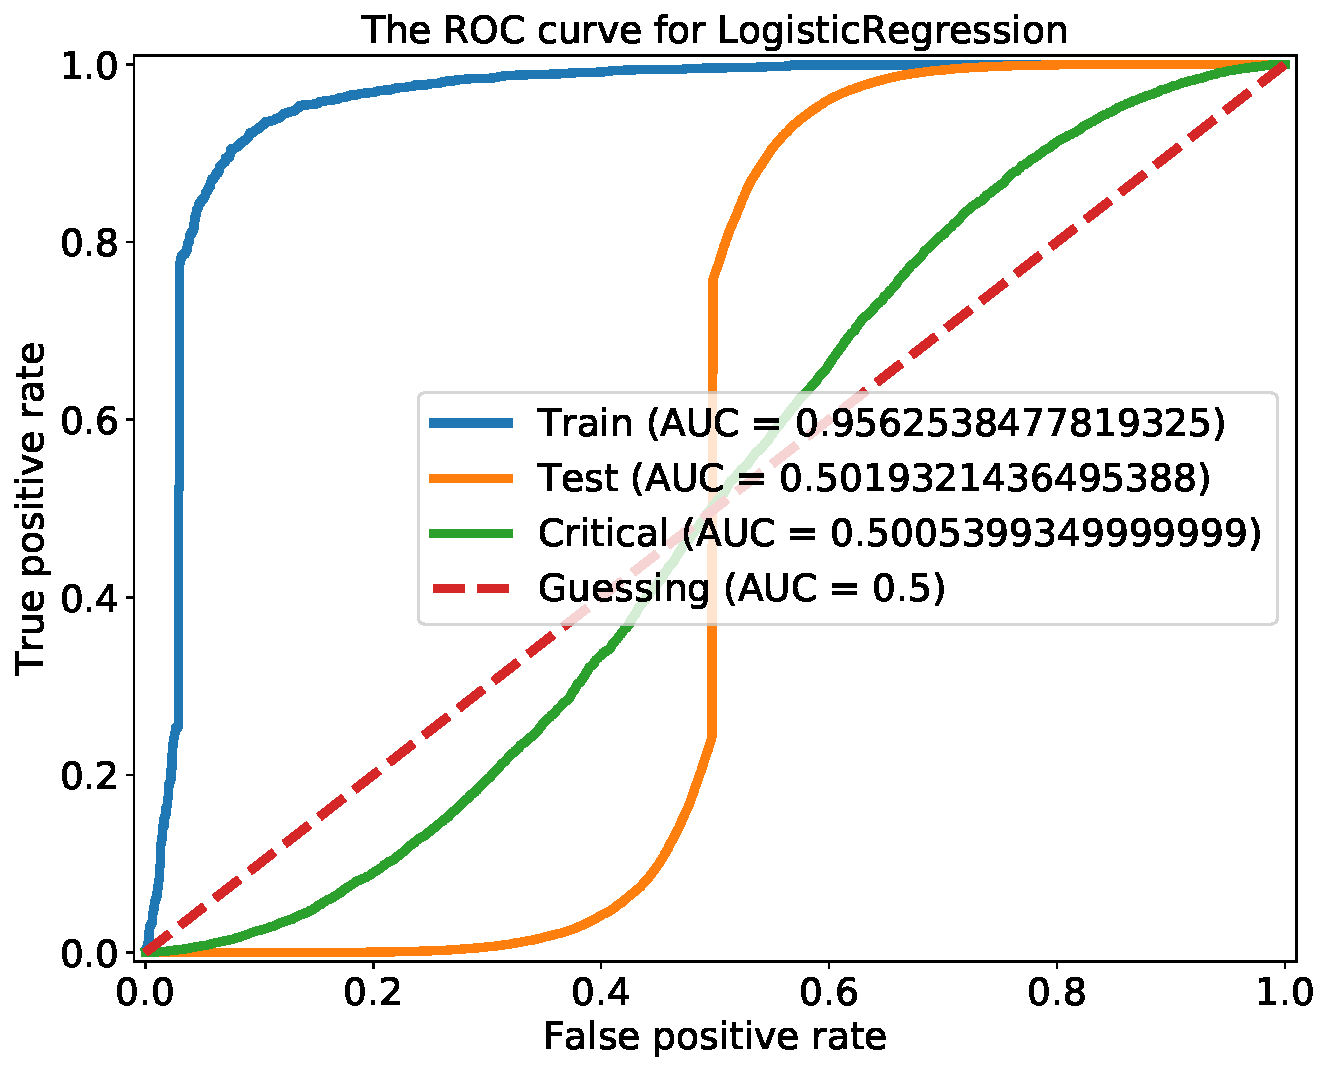
\includegraphics[scale=0.5]{latex/figures/logistic_roc_curve_nr.pdf}
\end{center}
\caption{figure text}
\label{fig:roc_nr}
\end{figure}

Logistic regression is not able to correctly fit the Ising model as it is not a linear model, and is, in the case with both Gradient Descent and Newton-Raphson as optimization methods, no better than just guessing.





%----------------------------------------------------------------
\subsection{Regression on Energy of Generalized Ising Model using Neural Networks}\label{sec:results NN reg}
%----------------------------------------------------------------
Accompanying notebook: \href{https://github.com/nicolossus/FYS-STK4155-Project2/blob/master/notebooks/nn_ising.ipynb}{nn\_ising.ipynb}.

Figure \autoref{fig:NN_reg} shows the R2-score different neural networks predicting the energy of the Ising model, using features produced by the Generalized Ising model.

\begin{figure}[H]
\centering
\subfloat[]{{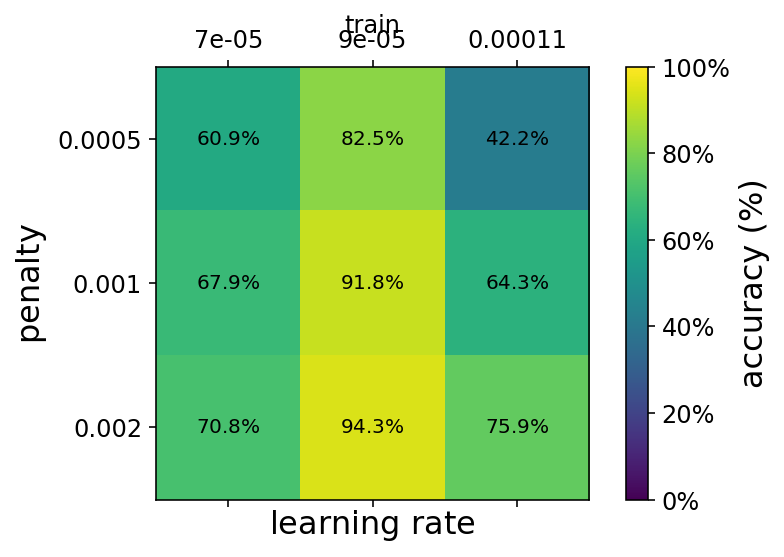
\includegraphics[scale=0.5]{latex/figures/NN_reg_train}}}
\qquad
\subfloat[]{{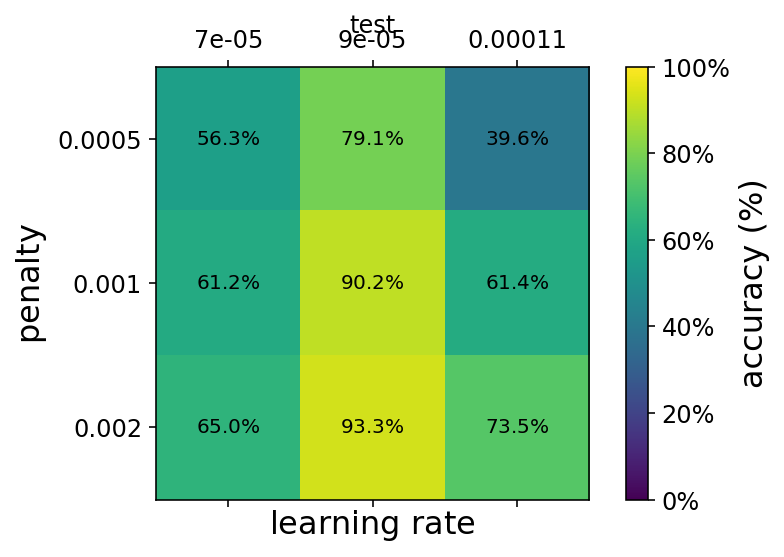
\includegraphics[scale=0.5]{latex/figures/NN_reg_test}}}
\caption{R2-score of several neural networks trained and tested on energies produced using the real Ising model \autoref{eq:ising 1D energy}, spin features produced using the generalized Ising model \autoref{eq:general}. All networks have a single hidden layer of 400 neurons, using $\tanh$ as activation, squared loss as cost function, and L2-regularization. They were trained using a grid search on learning rate and penalty}
\label{fig:NN_reg}
\end{figure}

As the real Ising model only include local coupling, only $80$ of the $1600$ features of the generalized model actually contribute to the energy. The interesting question to explore if the network is able to pick out the useful features and ignore the others. From the above figure, we see that the more heavily penalised models perform generally better. In the same manner that Ridge and Lasso help linear regression suppress features of less importance and reduce variance, the regularizing the network produces better models, presumably by suppressing the weights connecting to the redundant features. To go a step further, a model using $\mu = 9 \cdot 10^{-5}$ and $\lambda = 0.004$ was trained. This model yielded a $R^2$ score of 0.26. 

To elaborate the previous point, figure \autoref{fig:NN_CS} visualises the Connection Strength (CS), \autoref{eq:CS}, of all the inputs for models using learning rate $\mu = 9 \cdot 10^{-5}$ and penalties $0.0005$, $0.001$, $0.002$ and $0.004$. 

\begin{figure}[H]
\centering
\subfloat[]{{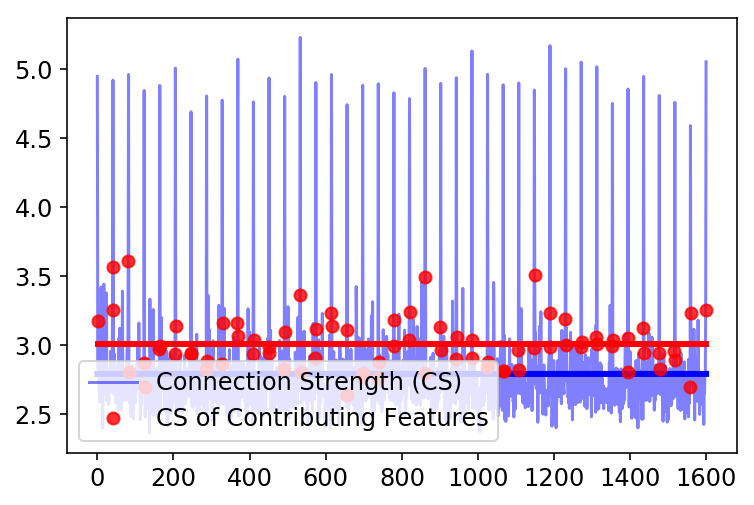
\includegraphics[scale=0.5]{latex/figures/pen1.png}}}
\qquad
\subfloat[]{{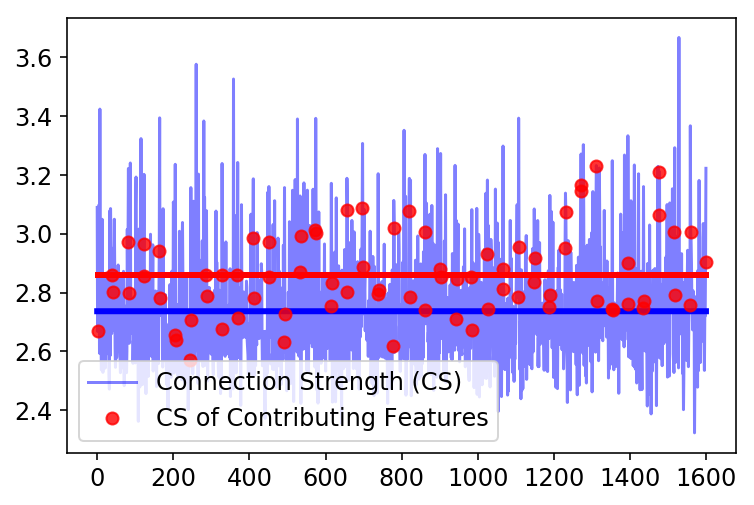
\includegraphics[scale=0.5]{latex/figures/pen2.png}}}
\qquad
\subfloat[]{{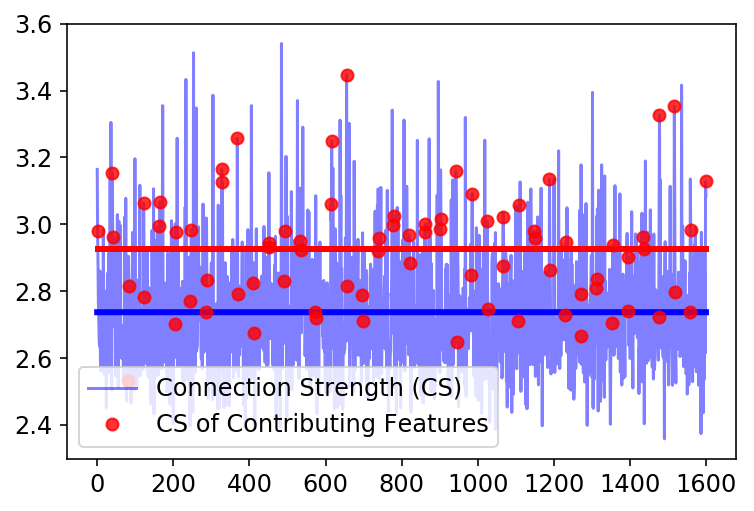
\includegraphics[scale=0.5]{latex/figures/pen3.png}}}
\qquad
\subfloat[]{{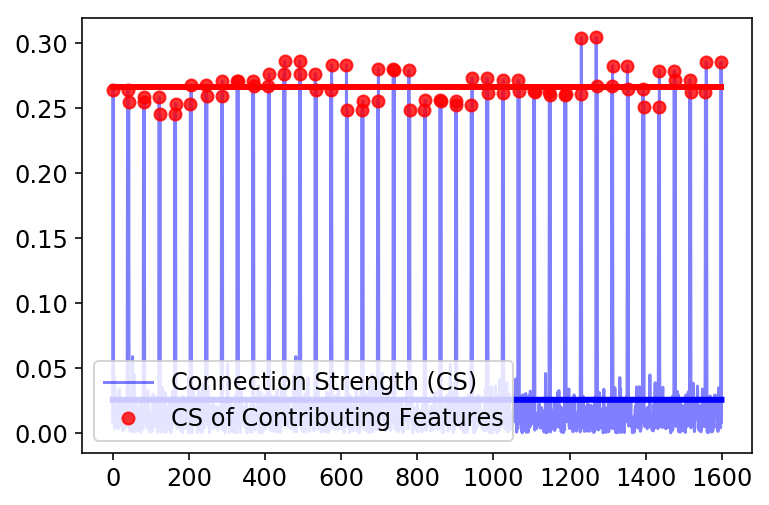
\includegraphics[scale=0.5]{latex/figures/pen4.png}}}
\caption{Connection strength \autoref{eq:CS} of all inputs for the models of learning rate $\mu = 9e-5$ and penalties $0.0005$, $0.001$, $0.002$ and $0.004$. The red dots highlights the CS of the features that contribute to the energy. The horizontal lines are the average CS of the two groups just described, respectively.}
\label{fig:NN_CS}
\end{figure}

As suspected, the increase in penalty raises the average CS of the inputs that contribute to the energy, making the network emphasize these inputs more. This ultimately yields a better model, until the penalty is raised to $0.004$. From the above figure, the contributing features are separated from the others more than ever. However, the weights have been shrunk to the point where the model is fairly desensitized to the features, with a CS of the order 0.3 instead of 3. Not too surprisingly, the model performed terribly, with a R2-score of $0.26$.

As a final note to the exploration of the learning behaviour, figure \autoref{fig:NN_learn} shows the $R^2$ score on validation data progressively as the network is trained.

\begin{figure}[H]
\centering
\subfloat[]{{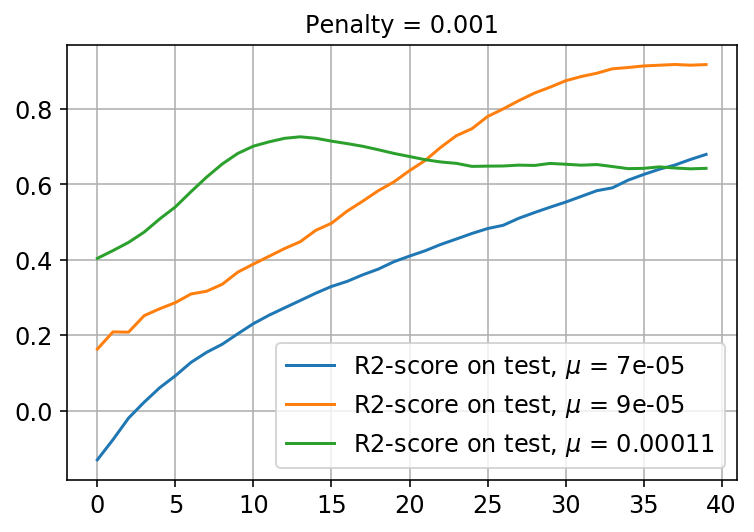
\includegraphics[scale=0.5]{latex/figures/NN_learn.png}}}
\caption{R2-score of neural networks evaluated on a independent validation set. The models all use penalty $\lambda = 0.001$, with learning rate $\mu = 7e-5$, $9e-5$ and $1.1e-4$.}
\label{fig:NN_learn}
\end{figure}

The plot highlights the typical problems of tuning learning rate: The model with the smallest learning rate is constantly improving, but never reaching its potential since the step size is too small. On the other hand, the one with the highest learning rate might be continuously skipping over its local minima after getting fairly close at first, resulting in gradually degrading results.   


%----------------------------------------------------------------
\subsection{Identifying 2D Ising Model Phases with Neural Networks}\label{sec:results NN reg}
%----------------------------------------------------------------

\autoref{fig:NN_class} shows the accuracy score of several neural networks trained and tested on the combined ordered and disordered set from Mehta et al. in \cite{Mehta_2019}. Additionally, the models were tested on the critical set to explore the generalizability of the models.

\begin{figure}[H]
\centering
\subfloat[]{{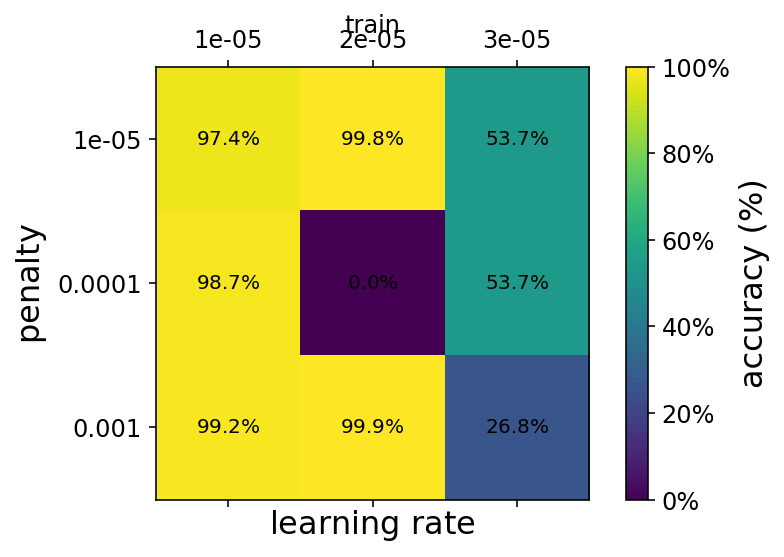
\includegraphics[scale=0.5]{latex/figures/NN_class1.png}}}
\qquad
\subfloat[]{{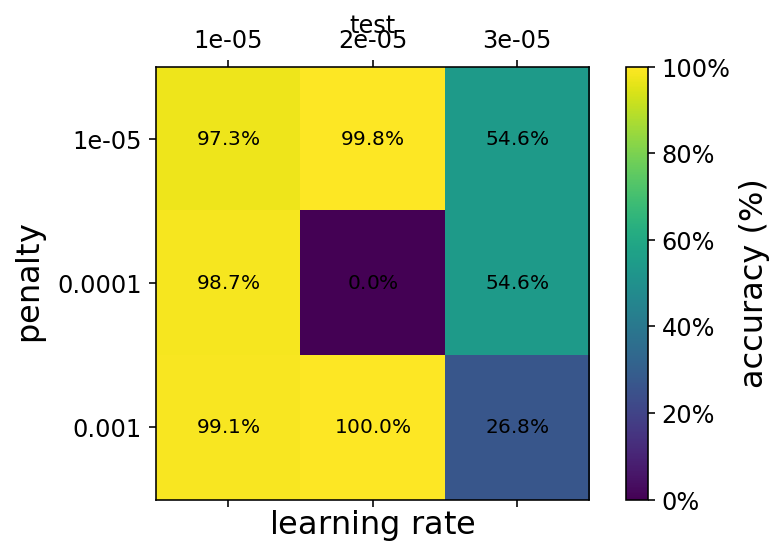
\includegraphics[scale=0.5]{latex/figures/NN_class2.png}}}
\qquad
\subfloat[]{{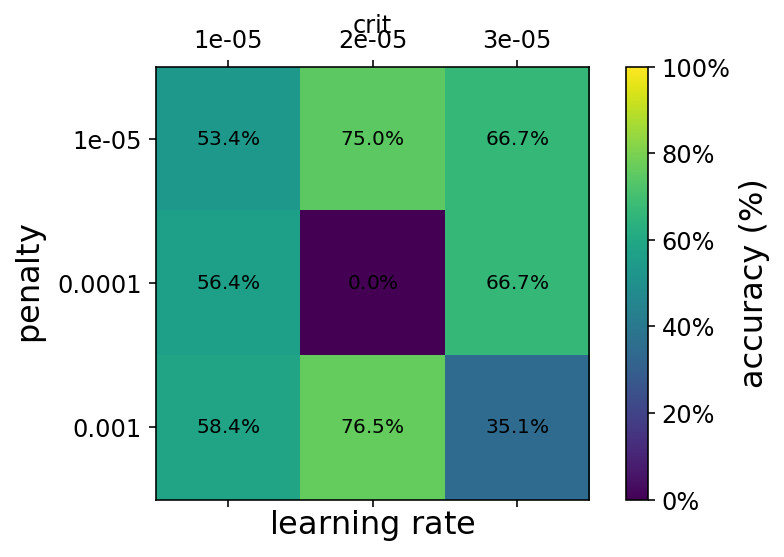
\includegraphics[scale=0.5]{latex/figures/NN_class3.png}}}
\caption{Accuracy score of several neural networks trained and tested on the combined ordered and disordered set from Mehta. Additionally, the models were tested on the critical set. All networks have a single hidden layer of 400 neurons, using sigmoid as activation on both the hidden layer and output. They were trained using a grid search on learning rate and penalty(L2-regularization)}
\label{fig:NN_class}
\end{figure}

An eye-catching result is the sudden ruination of one of the models, yielding a accuracy score of precisely zero. This is curious, since models with parameters in the same neighborhood yield sensible predictions. When the faulty model was trained, the program once encountered "value encountered in true divide". This is a weakness of the cross-entropy. If the network misclassifies a label, and if the network is very sure in its (mis)classification, the derivative of the cross-entropy becomes enormous. This will likely ruin the weights during the next GD step, and the model too.

The fluke aside, our model attained a maximum accuracy score of $100\%$ for the ordered/disordered data meant for testing, rivaling Mehta's model of $99.9\%$ accuracy. However, our models did not generalize as good on the critical data, attaining only an accuracy of $76.5\%$ as opposed to $95.9\%$. This could be that 400 nodes is not high enough complexity to capture the finer details needed to distinguish the critical states, or it could simply be because the learning rate and penalty was not chosen precise enough: Since the training is very expensive, our grid search is rather course.

\autoref{NN_misclass} highlights two states from the critical set that was misclassified by the best neural network trained on the ordered/disordered set.

\begin{figure}[H]
\centering
\subfloat[]{{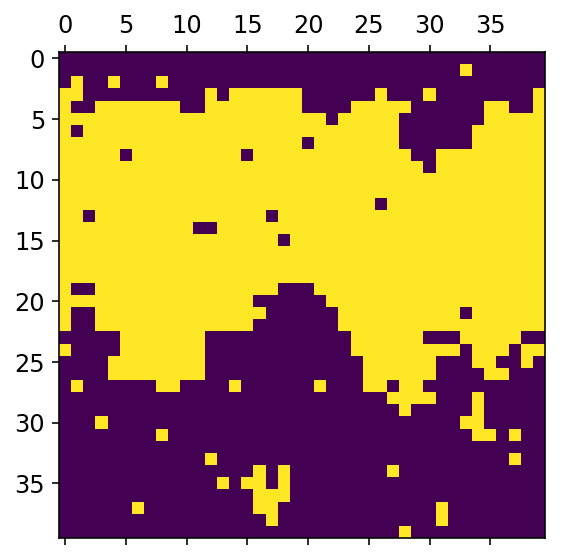
\includegraphics[scale=0.5]{latex/figures/NN_misclass.png}}}
\qquad
\subfloat[]{{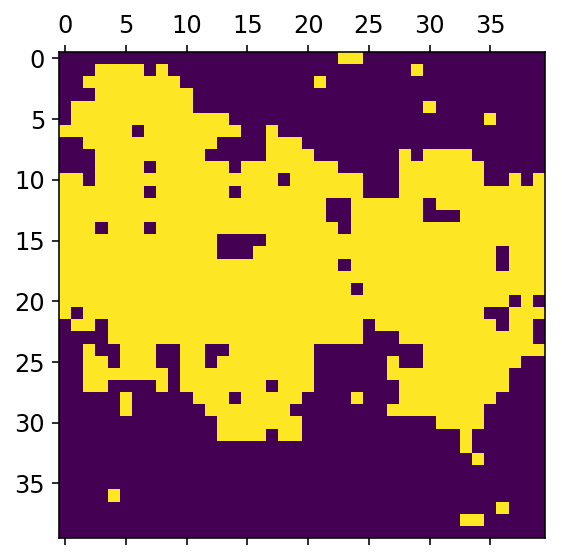
\includegraphics[scale=0.5]{latex/figures/NN_misclass2.png}}}
\caption{Examaple of two states from the critical set misclassified by the best network trained on the ordered/disordered set.}
\label{fig:NN_misclass}
\end{figure}

Purely visually, one can see where the ambiguity in classification occurs: The misclassified states looks locally ordered in some places and disordered in other. This ambiguity can be theorized to confuse the neural network and produce misclassification.  

